Los módulos en JavaScript, como en cualquier otro lenguaje de programación, ayudan a descomponer código en partes separadas más pequeñas. Este patrón ayuda a gestionar la creciente complejidad al mantener las preocupaciones separadas en sus partes independientes. En pocas palabras, los módulos ayudan a organizar el código.
\vspace{0.8cm}

Antes de ES6, esto se podía hacer usando diferentes archivos de script y luego cargando cada uno de ellos por separado con una etiqueta \code{<script>} en nuestro HTML. Esto tenía muchas desventajas, como mantener el orden correcto de los script para evitar romper accidentalmente cualquier código dependiente. Pero afortunadamente, ES6 trajo soporte para módulos con las palabras clave \code{import} y \code{export}, pero aún no son totalmente compatibles en todos los entornos (navegador y Node.js).
\vspace{0.8cm}

Webpack le permite escribir su código en módulos y unificarlos en uno o más paquetes. Webpack permite usar módulos y todas sus bondades sin preocuparse por el soporte. Además de JavaScript, también puede incluir otros tipos de archivos, incluidos (pero no limitados a) CSS, fuentes, imágenes, HTML, etc. y luego transformarlos en un formato aceptable. Webpack es extremadamente potente y se puede ampliar para hacer cosas impresionantes usando el concepto de loaders y pligins.
\vspace{0.8cm}

\subsubsection{Conceptos clave}
Webpack necesita una configuración básica para que funcione debidamente:

\begin{itemize}
  \item Entrada:
  Webpack utiliza el grafo de dependencias para decidir qué módulos deben agruparse. Esto significa que Webpack comienza desde un solo módulo y procesa todas sus dependencias directas e indirectas para formar el grafo de dependencia completo y luego agrupar todos los módulos necesarios.
  El punto de entrada determina desde dónde debe comenzar el paquete web para construir su gráfico de dependencia interna.\\
  Entrada del proyecto: \code{./src/app.js}
  \item Salida:
  La salida determina dónde se supone que el paquete web debe emitir los paquetes que crea y cómo los nombra. Este directorio también contendrá todos los archivos estáticos de la aplicación web que serán visibles al publico mediante el servidor Express.js.\\
  Salida del proyecto: \code{./www/bundle.js}
  \item Loaders
  Los loaders en el paquete web son los que le permiten manejar archivos que no son JavaScript (el empaquetador web solo comprende JavaScript). Los loaders leen varios tipos de archivos y los transforman en módulos válidos que webpack puede entender.
  \item Plugins
  Los plugins son la característica más poderosa de webpack, se utilizan para una amplia gama de tareas que los loaders no pueden realizar. Se utilizan  para la optimización de paquetes, minificación, emisión de estadísticas, etc.
\end{itemize}
\vspace{0.8cm}

\subsubsection{Babel Loader}
Babel ofrece el último soporte de sintaxis ECMAScript (ES5, ES6). Las librerías mas recientes insisten en que se utilicen las últimas ofertas de JavaScript para obtener un código más limpio y legible. Pero desafortunadamente nuestros navegadores no entienden la mayor parte de la sintaxis aquí es donde entra en juego Babel. Es responsable de convertir el código ES5 y ES6 en código comprensible por el navegador, básicamente compatibilidad con versiones anteriores. Las dependencias que necesita el proyecto son las siguientes:
\vspace{0.8cm}

\begin{itemize}
  \item babel-core: El motor principal de Babel para que sus dependientes trabajen.

  \item babel-preset-env: esta es la parte de soporte ES5, ES6

  \item babel-preset-react: Babel se puede usar en cualquier framework que necesite el soporte de sintaxis JS más reciente, en este caso es `React'.

  \item babel-loader: Un puente de comunicación entre Webpack y Babel
\end{itemize}
\vspace{0.8cm}

\lstinputlisting[style=ES6, caption=Fragmeno de configuración Babel.]{code/babelrc.json}

\lstinputlisting[style=ES6, caption=Fragmeno de configuración Webpack]{code/webpack.js}

\subsubsection{Webpack Dev Server}
La herramienta Webpack Dev Server ejecuta y sirve una compilación de nuestro proyecto, pero no lo escribe en el disco, lo hace en la memoria. En modo de desarrollo, este modulo hace que la aplicación se abra un navegador, y vuelva a cargar el navegador cuando detecte cambios en los archivos de los que depende la aplicación web.
\vspace{0.8cm}

\lstinputlisting[style=ES6, caption=Configuración Webpack Dev Server.]{code/webpack.dev.js}

Con la ayuda de Webpack se tiene la capacidad de importar estilos y componentes de React y hacer que algo no solo sea funcional, sino también estético. Los procesos de construcción pueden ser desalentadores, pero si se tiene una base sólida y se sabe cómo expandirla, pueden obtenerse buenos resultados.
\vspace{0.8cm}

% \begin{figure}[H]
%   \centering
%   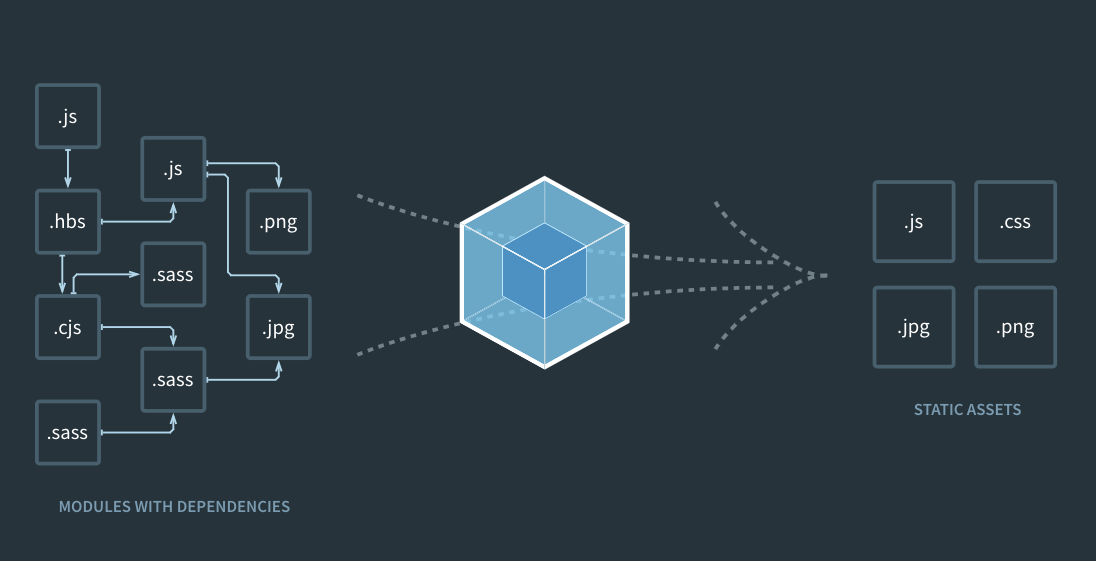
\includegraphics[width=1\textwidth]{webpack}
%   \caption{Imagen de la página oficial de Webpack donde se explica su concepto básico \cite{webpack}.}
% \end{figure}